\documentclass[11pt]{article}

\setlength{\oddsidemargin}{-0.25 in}
\setlength{\evensidemargin}{-0.25 in}
\setlength{\topmargin}{-0.9 in}
\setlength{\textwidth}{7.0 in}
\setlength{\textheight}{9.0 in}
\setlength{\headsep}{0.75 in}
\setlength{\parindent}{0.3 in}
\setlength{\parskip}{0.1 in}
\usepackage{epsf}
\usepackage{pseudocode}
\usepackage[shortlabels]{enumitem}
\usepackage{amsmath}
\usepackage{amssymb}
\usepackage{color}
\usepackage[normalem]{ulem}
\usepackage{graphicx}
\usepackage[export]{adjustbox}
\usepackage{wrapfig}
\pagenumbering{arabic}
\def\O{\mathop{\smash{O}}\nolimits}
\def\o{\mathop{\smash{o}}\nolimits}
\newcommand{\e}{{\rm e}}
\newcommand{\R}{{\bf R}}
\newcommand{\Z}{{\bf Z}}

\usepackage{amsmath}
\usepackage{amsfonts}
\usepackage{booktabs}

\usepackage{graphicx}
\usepackage{tikz}
\usetikzlibrary{arrows.meta}

%% display solutions or not
\newif\ifsol
\soltrue % comment out to hide solutions

\title{Section 11: Classification and Clustering}
\date{}
\author{CS 182 - Artificial Intelligence}
\begin{document}
\maketitle

\noindent Algorithms in machine learning fall under {\bf{supervised}} and {\bf{unsupervised}} approaches. In the former, we are given a set of inputs and labels/outputs, and would like to learn the relationship between them to guess label/output values for new data. In the latter, we are only given input values, and aim to find structure within them.

\section*{Supervised Learning}

Supervised learning can also be broken down into {\bf{parametric}} and {\bf{non-parametric}} approaches. Parametric algorithms, such as Naive Bayes or regression, rely on learning a set of parameters that define the classifier. Non-parametric algorithms, such as k-NN, rely directly on data rather than on a parameterized model. 

\subsection*{Naive Bayes}

Naive Bayes can be thought of as a {\bf{probabilistic inference algorithm}} over a special case of a Bayes Net that is applied to classification. The model is made of an unknown variable $Y$ representing the possible classes, which causes a collection of emission variables $E_1$, $E_2$, $\dots$, $E_n$. We make a (``naive'') assumption that each of the emissions is conditionally independent of one another given $Y$. While this may not be true for most applications, it still results in a simple and useful algorithm. Finally, given the emissions, we can calculate classification probabilities by inference over the Bayes Net:
\[
P(Y | x_1, \ldots, x_n) \propto P(Y, x_1, \ldots, x_n) = P(Y) \prod_{i=1}^n P(x_i|Y)
\]
To build up this network from labeled data, we can count the frequencies of occurrence of observing $(x_i, Y)$ for each $x_i$ and normalize to construct conditional probabilities. Improvements on this approach involve {\bf{smoothing}}, which is discussed further down.


\subsection*{Regression}

When the output variable $y$ is continuous rather than discrete, we can perform regression. First, a {\bf{model}} $h_{\theta}$ is chosen to describe the input-output relationship, where the {\bf{model parameters}} $\theta$ are calculated by optimizing over a {\bf{loss function}} $L$ on the training data. For instance, if we assume that the underlying model is {\bf{linear}}, we choose $h_{\theta}(f^{(i)}) = \theta^T f^{(i)}$ for every $i$th data vector. Often, a quadratic loss function is chosen. This is both intuitive, but also theoretically supported -- a quadratic is the {\bf{maximum likelihood estimate}} of the data given the model parameters, under the assumption of i.i.d. Gaussian noise in the data. Overall, the optimization problem to solve {\bf{linear regression}} would be:
\[
\min_{\theta} \; \; \sum_{i = 1}^m (\theta^T f^{(i)} - y^{(i)})^2
\]
There are other possible loss functions, such as:
\begin{itemize}
    \item \bf{absolute ($L_1$) loss}: $L = |h_{\theta}(f) - y|$
    \item \bf{deadband loss}: $L = \max(0, |h_{\theta}(f) - y| - \epsilon)$
\end{itemize}

\noindent {\bf{Logistic regression}} is a variant of regression designed for binary classification (where the output variable does assume discrete values $0$ and $1$). Instead of using the linear function $h_{\theta}(f) = \theta^T f$, we apply a sigmoid:
\[
h_{\theta} = \frac{1}{1 + e^{-\theta^T f}}
\]
Similarly to linear regression, we choose a loss function, pose an optimization problem, and solve for the optimal parameters $\theta$. 

\noindent While linear regression with a quadratic loss is {\bf{convex}} and has a closed-form solution, most of these optimization problems are non-convex and are solved with {\bf{stochastic gradient descent}}. Finally, after an optimization approach is applied and the model parameters $\theta$ are determined, we can guess the output of new data $f$ by calculating $h_{\theta}(f)$ (for the binary logistic case, rounding it to 0 or 1).




\subsection*{k-Nearest Neighbors}
This is a simple {\bf{non-parametric}} classification approach which assigns a label to a new point by choosing the most common class of the $k$ closest neighboring points. Variations on this algorithm might give a weighting scheme to the $k$ labels rather than choosing the most common value. 


\noindent When designing an ML algorithm, the available data is usually broken up into the {\bf{training data}}, which is used to train the classifier, and the {\bf{test data}}, which is used to evaluate the classifier and can in no way be viewed or used beforehand. \noindent This division of datasets allows to deal with two issues:
\begin{enumerate}
    \item {\bf{Overfitting}} occurs when a classifier is trained for very high (near 100\%) training accuracy, but is not able to {\bf{generalize}} to the testing data, and has low test accuracy.
    \begin{enumerate}
        \item {\bf{Smoothing}} is used in discrete problems to cause more gradual updates to probabilities. For instance, one example of overfitting would be giving zero probabilities to all words not in the training set, which can be mitigated with {\bf{Laplace smoothing}}:
        \begin{align*}
        &\text{standard probability:} \; \; P_{ML}(x) = \frac{count(x)}{N} \\
        &\text{with smoothing:} \; \; P_{LAP, k}(x) = \frac{count(x) + k}{N + k|X|}
        \end{align*}
        \item {\bf{Regularization}} is used in continuous problems such as regression. For instance, an example of overfitting would be using a high-order polynomial that goes through all training data points. The addition of a regularization term to the loss function places an analytic penalty on problem parameters to encourage smaller values or sparsity:
        \begin{align*}
        &\text{standard loss function:} \; \; loss(f^{(i)}, y^{(i)}, \theta) = (\theta^T f^{(i)} - y^{(i)})^2 \\
        &\text{with $L_2$-regularization:} \; \; loss(f^{(i)}, y^{(i)}, \theta) = (\theta^T f^{(i)} - y^{(i)})^2 + \lambda ||\theta||_2^2 \\
        &\text{with $L_1$-regularization:} \; \; loss(f^{(i)}, y^{(i)}, \theta) = (\theta^T f^{(i)} - y^{(i)})^2 + \lambda ||\theta||_1
        \end{align*}
    \end{enumerate}
    \item Sometimes algorithms depend on a choice of {\bf{hyperparameters}}, which must be decided outside of the training process. There are a couple common approaches to tuning:
    \begin{enumerate}
        \item Part of the training data is taken to be the {\bf{held-out dataset}}. For each hyperparameter value, the classifier is trained with the rest of the training data and tested on the held-out data, and the one with the highest accuracy is chosen.
        \item If there are $m$ possible values for a hyperparameter, {\bf{cross-validation}} divides the training data into $m$ sections. For the $i$th value, the $i$th section is chosen to be the tuning test set and the others are chosen to be the tuning training sets. After evaluating all hyperparameter values, the one with the highest tuning test accuracy is chosen.
    \end{enumerate}
\end{enumerate}


\section*{Unsupervised Learning}

Unsupervised learning algorithms focus primarily on clustering, dimensionality reduction, anomaly detection, or other ways of inferring data structure without labels. The algorithms we have discussed all fall under clustering.

\noindent {\bf{K-means}} is a {\bf{centroid-based}} clustering algorithm. First, initialize $k$ cluster centroids. Then, iteratively:

\noindent Assign each point to nearest cluster centroid:
\[
a_i = \text{argmin}_k \; \text{dist}(x_i, c_k), \;\; i = 1, \dots, N
\]

\noindent Recompute the $k$th cluster centroid by taking the mean of the points assigned to cluster $k$:
\[
c_k = \frac{1}{|a_i \;:\; a_i = k|} \sum_{(i \;:\; a_i = k)} x_i, \;\; k = 1, \dots, K
\]


\noindent {\bf{Agglomerative clustering}} and {\bf{divisive clustering}} are both {\bf{connectivity-based}} clustering algorithms. The former iteratively constructs larger clusters from smaller clusters. The latter iteratively breaks down large clusters into smaller clusters.

\noindent {\bf{Choosing K:}} The outcome of all of these algorithms vary on the chosen number of clusters. Some common approaches for choosing $k$ are:
\begin{itemize}
    \item We can plot the average of the distances from each point to its cluster's centroid. Then, it is reasonable to choose the smallest value of $k$ for which this ``error'' flattens out.
    \item {\bf{Silhouette diagrams}} are plots of the measure
    \[
    m_i = \frac{(b_i - a_i)}{\max(a_i, b_i)}
    \]
    where $a_i$ is the mean distance from the point $x_i$ to all points in its cluster, and $b_i$ is the mean distance from $x_i$ to all points in the neighboring (``next best'') cluster.
\end{itemize}



%\begin{figure}[ht]
%\renewcommand{\labelenumii}{\arabic{enumii}.}
%\setlength{\parindent}{0pt}
%    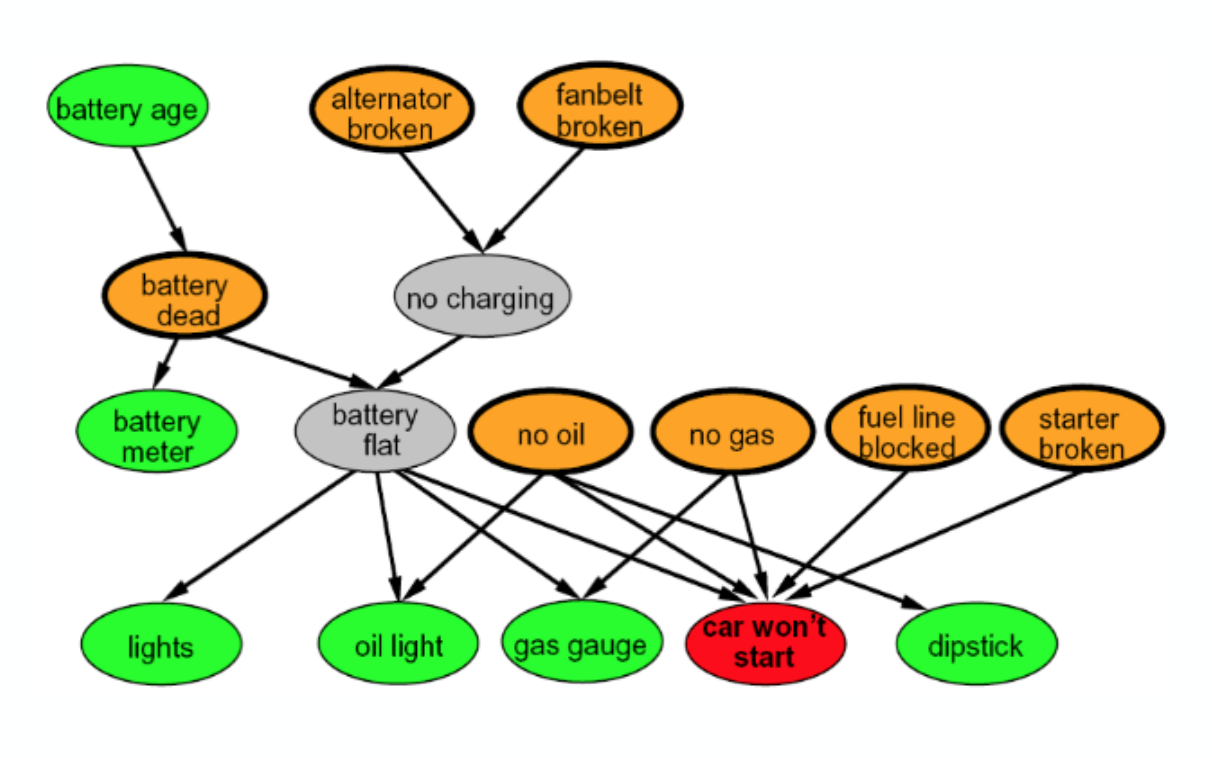
\includegraphics[scale=0.4]{figs/carrepair}
%    \caption{Conditional implications example (left), example conditional probability tables (center), and example bayes net for car repair (right)}
%    \label{fig:bayes}
%\end{figure}



%%%%%%%%%%%%%%%%%%%%%%%%%%%%%%%%%%%%%%%%%%%%%%%%%%%%%%%%%%%%%%%%%%%%%%%%%%%%%%%%
%%%%%%%%%%%%%%%%%%%%%%%%%%%%%%%%%%%%%%%%%%%%%%%%%%%%%%%%%%%%%%%%%%%%%%%%%%%%%%%%

\newpage
\section*{Exercises:}
\begin{enumerate}


\item{{\bf{Silhouette Diagrams.}}}

Suppose we are trying to cluster an unlabeled dataset. We apply k-means with $k = 3$, and are evaluating the clusters with a with a silhouette diagram.
\begin{enumerate}
    \item Suppose that for a certain point $x_i$, $a_i << b_i$. What will be the approximate value of $m_i$, and what does this imply about the clustering of $x_i$? \\
    \ifsol
        {\color{blue} If $a_i$ is small relative to $b_i$, this is a good clustering of $x_i$, since it is (on average) much closer to points in its own cluster than the next best cluster. The measure $m_i$ will be close to 1.}
    \else
        \vspace{1cm}
    \fi
    \item Suppose that for a certain point $x_i$, $a_i \approx b_i$. What will be the approximate value of $m_i$, and what does this imply about the clustering of $x_i$? \\
    \ifsol
        {\color{blue} If $a_i$ is similar to $b_i$, this is not a very good clustering of $x_i$, since it is about the same distance away from points in its own cluster as those in the next best cluster. The measure $m_i$ will be close to 0.}
    \else
        \vspace{1cm}
    \fi
    \item Suppose that for a certain point $x_i$, $a_i >> b_i$. What will be the approximate value of $m_i$, and what does this imply about the clustering of $x_i$? \\
    \ifsol
        {\color{blue} If $a_i$ is much greater than $b_i$, this is an incorrect clustering of $x_i$, since it is much farther from points in its own cluster as those in the next best cluster (this situation should be impossible with k-means). The measure $m_i$ will be close to -1.}
    \else
        \vspace{1cm}
    \fi
\end{enumerate}


\item{{\bf{Regression.}}}

You are working for a hospital, and are given a dataset of patient information with hundreds of continuous features (height, weight, blood pressure, etc) along with whether the patient has diabetes. Your goal is to predict whether incoming patients will have diabetes.

\begin{enumerate}
\item Formalize the problem as an optimization problem using logistic regression. \\
\ifsol
    {\color{blue} Let $f^{(i)}$ be the vector of features for the $i$th patient, $y^{(i)}$ be the true outcome (diabetes or no diabetes) for each patient, and $\theta$ be the parameters we are learning. Then, if we use a sum-of-squared-error loss function, we are trying to solve the problem:
    \[
    \hat{\theta} = \text{argmin}_{\theta} \; \sum_{i} (\frac{1}{1 + e^{-\theta^T f^{(i)}}} - y^{(i)})^2
    \]
    
    }
\else
    \vspace{1cm}
\fi

\item Write down the formula your model would use to compute the probability that a patient has diabetes. \\
\ifsol
    {\color{blue} Once the parameters $\theta$ are learned by solving the problem above, a new patient's probability of having diabetes given a feature vector $f$ will be
    \[
    P(y | f) = \frac{1}{1 + e^{-\theta^T f}}
    \]
    .}
\else
    \vspace{1cm}
\fi

\item Suppose you are now trying to estimate blood pressure using linear regression on the 20 features you consider most important. If you calculate a regression model on a training set of 12 patients, what (approximately) will be your training set error? \\
\ifsol
    {\color{blue} In this problem, we have 20 ``unknowns'' (the parameters $\theta$ and only 12 ``equations'' (the training data). Therefore, unless the training data contains equations which exactly contradict each other, this is an under-determined system, and we can choose $\theta$ such that all the total error is 0. This is an example of overfitting.}
\else
    \vspace{1cm}
\fi
\end{enumerate}

\newpage

\item{\bf{Naive Bayes}}

In this problem, we will be using Naive Bayes to predict the probability that a given email is spam or not spam (ham). We assume a model in which an underlying unobserved state $y$ (spam/ham) creates emissions (words) $w_1, \ldots, w_n$. We use a bag-of-words approach to model text -- the ordering of words within a sentence is ignored. Then, $P(Y)$ is the prior probability across states $Y$, and  $p(w_i|Y)$ are the conditional probabilities of seeing a word $w_i$ given $Y$. For the problems, start by assuming a uniform distribution over $Y$, and use the following conditional probability table over words:

% Please add the following required packages to your document preamble:
% \usepackage{booktabs}
\begin{table}[h!]
\centering
\begin{tabular}{@{}lll@{}}
\toprule
        & $p(w|ham)$ & $p(w|spam)$ \\ \midrule
CS182   & 0.05     & 0.01      \\
friend  & 0.02     & 0.04      \\
need    & 0.01     & 0.01      \\
on      & 0.02     & 0.02      \\
our     & 0.02     & 0.02      \\
project & 0.007    & 0.003     \\
start   & 0.01     & 0.03       \\
to      & 0.01     & 0.01      \\
you     & 0.01     & 0.015     \\
we      & 0.01     & 0.015     \\
working & 0.01     & 0.03      \\
...     & ...      & ...      \\ \bottomrule
\end{tabular}
\end{table}

\begin{enumerate}
\item
What is the probability of seeing the following spam email: ``we need you on our project friend''?\\
\ifsol
\textcolor{blue}{\[
p(email|spam) = 0.015*0.01*0.015*0.02*0.003*0.04 = 5.4 *10^{-12}
\]}
\else
    \vspace{1cm}
\fi

\item
What is the probability that the following text is spam: ``start CS182 project''?\\
\ifsol
\textcolor{blue}{\begin{align*}
p(email|ham) &= 0.01 * 0.05 * 0.007 = 0.0000035 \\
p(email|spam) &= 0.03 * 0.01 * 0.003 = 0.0000009\\
p(spam|email) &\propto 0.5 * 0.0000009\\
p(ham|email) &\propto 0.5 * 0.0000035%\frac{0.5 * 0.0000009}{0.0000009+0.0000035} = 0.102
\end{align*}
We can normalize this and get a probability for $p(spam|email) = 0.205$.
}
\else
    \vspace{1cm}
\fi


\item We now consider a fresh inbox for which we have no previous data. We want to build a new classifier from scratch. The inbox right now contains three emails:
\begin{enumerate}
\item [spam:] ``I am only prince''
\item [spam:] ``I will send money''
\item [ham:] ``I will send you the review for it''
\end{enumerate}
Determine the prior over Y (spam/ham), fill in the probability table below, and calculate the probabilities that the email ``I will send'' is spam/ham.\\
\ifsol
\begin{table}[h!]
\centering
\begin{tabular}{@{}lllll@{}}
\toprule
       & freq ham & $p(w|ham)$ & freq spam & $p(w|spam)$ \\ \midrule
am     & 0        & 0          & 1         & 1/8         \\
for    & 1        & 1/8        & 0         & 0           \\
I      & 1        & 1/8        & 2         & 2/8         \\
it     & 1        & 1/8        & 0         & 0           \\
money  & 0        & 0          & 1         & 1/8         \\
only   & 0        & 0          & 1         & 1/8         \\
prince & 0        & 0          & 1         & 1/8         \\
review & 1        & 1/8        & 0         & 0           \\
send   & 1        & 1/8        & 1         & 1/8         \\
the    & 1        & 1/8        & 0         & 0           \\
you    & 1        & 1/8        & 0         & 0           \\
will   & 1        & 1/8        & 1         & 1/8         \\ \bottomrule
\end{tabular}
\end{table}
\else
\begin{table}[h!]
\centering
\begin{tabular}{@{}lllll@{}}
\toprule
       & freq ham & $p(w|ham)$ & freq spam & $p(w|spam)$ \\ \midrule
am     &         &           &          &          \\
for    &         &         &          &            \\
I      &         &         &          &          \\
it     &         &         &          &            \\
money  &         &           &          &          \\
only   &         &           &          &          \\
prince &         &           &          &          \\
review &         &         &          &            \\
send   &         &         &          &          \\
the    &         &         &          &            \\
you    &         &         &          &            \\
will   &         &         &          &          \\
\bottomrule
\end{tabular}
\end{table}
\fi

\ifsol
\textcolor{blue}{We can determine the prior by counting the number of emails from each category:  $p(spam) = 2/3$ and $p(ham) = 1/3$. To construct the table, we count the word frequencies and normalize by the number of words. Using this table, we can take the same approach as before:}
\begin{align*}
p(email|ham) &= \left(1/8\right)^3 = 0.00195\\
p(email|spam) &= 2/8 * 1/8 * 1/8 = 0.0039\\
p(ham|email) &\propto \frac{1}{3} * 0.00195 = 0.00065\\%\frac{0.00195}{0.00195+0.0039} = 0.111\\
p(spam|email) &\propto \frac{2}{3} * 0.0039 = 0.0026\\%\frac{0.0039}{0.00195+0.0039} = 0.444
\end{align*}

\textcolor{blue}{Normalizing this yields 0.2 and 0.8 probabilities for the two classes respectively.}
\else
    \vspace{1cm}
    \newpage
\fi

\item For long texts, you will need to multiply many numbers smaller than 1. This can cause implementation problems, where all of the predicted probabilities are so small that they are numerically rounded to zero. What can you do to address this issue? Why does it work?\\
\ifsol
\textcolor{blue}{In order to avoid those issues, you can add up the log-probabilities. This works because $$P(Y) \prod_{i=1}^n P(w_i|Y) = e^{\log (P(Y) \prod_{i=1}^n P(w_i|Y))} = e^{\log P(Y) \sum_{i=1}^n \log P(w_i|Y)}$$}
\else
    \vspace{1cm}
\fi

\item Use your classifier to predict the emails ``Will you send the review'' and ``Please send the review''.\\
\ifsol
\textcolor{blue}{Those two are special cases. Since $p(review|spam)=0)$, we have a 0 probability for the whole term. The word ``please'' does not occur in the table and with the current approach, we can't compute the probabilities.} \newpage
\else
    \vspace{1cm}
\fi


\item Repeat task (c) with laplace smoothing and $k=1$.\\

\ifsol
\textcolor{blue}{
\begin{table}[h!]
\centering
\begin{tabular}{@{}lllll@{}}
\toprule
       & freq ham & $p(w|ham)$ & freq spam & $p(w|spam)$ \\ \midrule
am     & 1        & 1/20       & 2         & 2/20         \\
for    & 2        & 2/20       & 1         & 1/20           \\
I      & 2        & 2/20       & 3         & 3/20         \\
it     & 2        & 2/20       & 1         & 1/20           \\
money  & 1        & 1/20       & 2         & 2/20         \\
only   & 1        & 1/20       & 2         & 2/20         \\
prince & 1        & 1/20       & 2         & 2/20         \\
review & 2        & 2/20       & 1         & 1/20           \\
send   & 2        & 2/20       & 2         & 2/20         \\
the    & 2        & 2/20       & 1         & 1/20           \\
you    & 2        & 2/20       & 1         & 1/20           \\
will   & 2        & 2/20       & 2         & 2/20         \\
\bottomrule
\end{tabular}
\end{table}
\begin{align*}
p(email|ham) &= \left(1/10\right)^3 = 0.001\\
p(email|spam) &= 3/20 * 2/20 * 2/20 = 0.0015\\
p(ham|email) &\propto \frac{1}{3} * 0.001 = 0.000333...\\%\frac{0.00195}{0.00195+0.0039} = 0.111\\
p(spam|email) &\propto \frac{2}{3} * 0.0015 = 0.001\\%\frac{0.0039}{0.00195+0.0039} = 0.444
\end{align*}
Normalizing this yields 0.25 and 0.75 probabilities for the two classes respectively.
}
\else
\begin{table}[h!]
\centering
\begin{tabular}{@{}lllll@{}}
\toprule
       & freq ham & $p(w|ham)$ & freq spam & $p(w|spam)$ \\ \midrule
am     &         &           &          &          \\
for    &         &         &          &            \\
I      &         &         &          &          \\
it     &         &         &          &            \\
money  &         &           &          &          \\
only   &         &           &          &          \\
prince &         &           &          &          \\
review &         &         &          &            \\
send   &         &         &          &          \\
the    &         &         &          &            \\
you    &         &         &          &            \\
will   &         &         &          &          \\
\bottomrule
\end{tabular}
\end{table}
\fi

\item What are other possible features you can consider?\\
\ifsol
\textcolor{blue}{We can incorporate any features that are representative of spam emails in addition to word frequencies. Examples are
\begin{itemize}
\item ``Online Pharmacy''
\item Mentions large quantities of money
\item Sent by an unknown address with many numbers
\item Subject is all capitals
\item Email body has low ratio of text to images	
\item ``One hundred percent guaranteed''	
\item ``Prestigious Non-Accredited Universities''
\end{itemize}
Another approach is to also count occurrences of longer phrases (called n-grams).}
\else
\fi

\end{enumerate}


\end{enumerate}
\end{document}
